%!TEX root = ../DSGEnotes.tex
\section{数值求积}
\label{sec:numerical-integration-ncrule}

我们常常需要计算一个定积分的值,如
\begin{equation*}
  \int_{a}^{b} f(x) \, \mathrm{d}x,
\end{equation*}
若直接用解析法求解较为困难,则常常采取数值积分(numerical integratation)\index{numerical integration \dotfill 数值积分}的思路,将积分式转化为有限个方程求和的方式做近似求解,如
\begin{equation}
  \label{eq:nint-num-integ-def}
  \int_{a}^{b} f(x) \, \mathrm{d} x \approx \sum_{n=1}^{N} w_{n} f \left( x_{n} \right),
\end{equation}
也即,我们在原方程的取值区间$[a,b]$中抽取$N$个点,$n=0,1,\ldots,N$的$x_{n}$值代回方程中对应值$f \left(x_{n} \right)$。$w_{n}$表示相应的权重系数。

因此,数值积分也常常称为数值求积(numerical quadrature)\index{numerical quadrature \dotfill 数值求积}。集合$\left\{ x_{n} \right\},\left\{ w_{n} \right\}$常常称为求积点(quadrature points)\index{quadrature points \dotfill 求积点}集合和求积权重(quadrature weights)\index{quadrature weights \dotfill 求积权重}集合;合适的选取$\left\{ x_{n} \right\},\left\{ w_{n} \right\}$的算法称为求积法则(quadrature rule)\index{quadrature rule \dotfill 求积法则}。对于同一个积分求解问题\eqref{eq:nint-num-integ-def}往往存在一系列法则;评价不同法则之间好坏的标准在于,看哪个法则能用最少的样本点$N$来对\eqref{eq:nint-num-integ-def}作出最精确的近似,同时确保计算成本可控,如编程难度、计算时间等。

先从最基本的牛顿——寇特斯法则开始介绍。

\subsection{牛顿——寇特斯法则}
\label{sec:nint-nc-rule}
近似求解积分问题\eqref{eq:nint-num-integ-def}的基本思路是,在区间$[a,b]$中找到一个多项式方程$P(x)$来近似$f(x)$。由于多项式的求和计算往往较为简单(多项式的介绍见第\ref{sec:poly}节),这会简化\eqref{eq:nint-num-integ-def}RHS的计算时间。我们将这种思路称为牛顿——寇特斯(求积)法则(Newton—Cotes Rule)\index{Newton—Cotes Rule \dotfill 牛顿——寇特斯法则}。牛顿——寇特斯法则随着多项式的次(degree, order)而呈层级特征:使用$p$次多项式的牛顿——寇特斯法则可称为$p$阶牛顿——寇特斯法则。

如果$f$不是多项式,那么在$[a,b]$区间内寻找近似多项式$P(x)$会较为困难。一个近似方案是将空间$[a,b]$划分为$N$个子区间(对应$N+1$个点),在每个子空间中分别寻找可以近似$f$的多项式,进而将多个多项式加权求和,作为整个空间中$f$的近似方程。$N$越大,子空间的个数越多,划分就越精细,每个子空间中的近似就越精确,进而整个空间中的近似求积就越精确。

\subsubsection{矩形法则}
\label{sec:ninc-nc-rectangular-rule}
我们先从$p=0$的情况开始理解牛顿——寇特斯法则,根据黎曼求和(Riemann sums),我们可以将方程$f(x)$理解为一组矩形的集合,对$f(x)$在区间$[a,b]$中求积就是求曲线下方的面积,近似等于各个矩形面积的和。随着$N$趋近于无穷大,每个矩形的宽度无限接近于$0$,近似就越精确。

在每个子空间中分别用$1$个$p=0$次多项式来近似$f$,$0$次多项式是个常数,换句话说我们在每个子空间中用一个常数来近似$f$。这又称为矩形求积法则(rectangular quadrature rule)\index{rectangular (quadrature) rule \dotfill 矩形(求积)法则}。

\begin{figure}[htbp]
   \caption{矩形法则$(N=4)$}
  \centering
  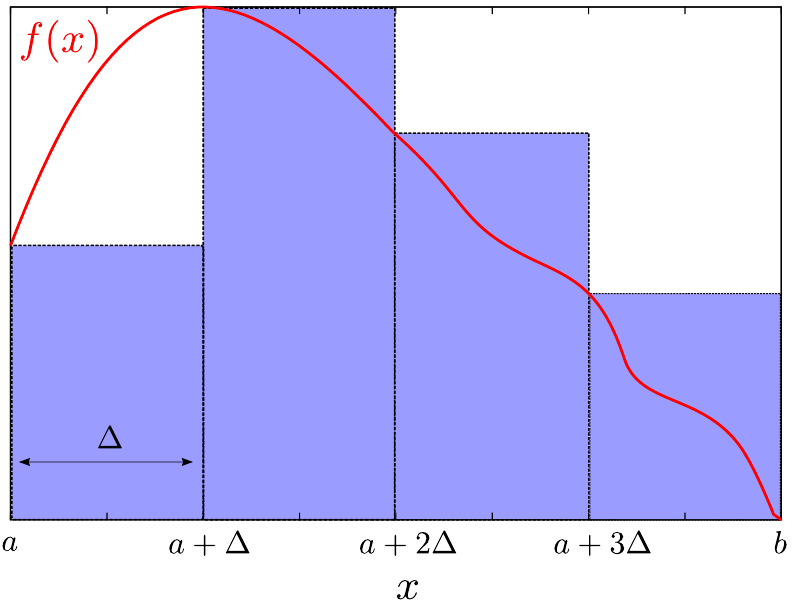
\includegraphics[width=8cm]{./Figures/20180227-rectangular-rule-example.png}
  \label{fig:ninc-nc-rectangular-rule}
%
%  \small{Source: PBOC.}
\end{figure}
图\ref{fig:ninc-nc-rectangular-rule}绘出了$N=4$情况下,利用矩形法则对$\int_{a}^{b} f(x) \, \mathrm{d}x$的近似。不难看出,将区间$[a,b]$划分为$N$个等宽子区间,每个子区间的宽度都是$\Delta = \left(b - a \right)/N$。最左侧第一个矩形,左边长(高)为$f(a)$,宽为$\Delta$,对应面积为$f(a) \cdot \Delta$。
左数第二个矩形,左边长(高)为$f \left( a+\Delta \right)$,宽也是$\Delta$,面积为$\left( a+\Delta \right) \cdot \Delta$,以此类推直到第$N=4$个矩形为止。将这些子区间中矩形的面积加总,可得矩形法则的近似表达式
\begin{equation*}
    \mathcal{I}_{N=4}^{rect}
    %\mathcal{N}_{N=4}^{rect}
    \approx
    f(a) \cdot \Delta
    + f \left(a + \Delta \right) \cdot \Delta
    + f \left(a + 2 \Delta \right) \cdot \Delta
    + f \left(a + 3 \Delta \right) \cdot \Delta,
\end{equation*}
扩展到更一般的$N \in \mathcal{N}$的情况,利用$N$段矩形法则对积分$\int_{a}^{b} f(x) \, \mathrm{d} x$的近似为
\begin{equation}
  \label{eq:ninc-nc-rectangular-rule}
  \mathcal{I}_{N}^{rect} = \sum_{n=0}^{N-1} f \left( a + n \cdot \Delta \right) \cdot \Delta.
\end{equation}

矩形法则\eqref{eq:ninc-nc-rectangular-rule}成为对\eqref{eq:nint-num-integ-def}的近似求积法则之一:
\begin{itemize}
  \item 求积权重集合$\left\{ w_{n} \right\}_{n=0}^{N-1}$对应$w_{n} \equiv \Delta \, \forall \, n$,
  \item 求积点集合$\left\{ x_{n} \right\}_{n=0}^{N-1}$对应$x_{n} = a + n \cdot \Delta, \, n = 0,1,\ldots,N-1$。
\end{itemize}

值得注意的是,在矩形法则下,我们只需要左边长,从而无需计算$f(b)$。


\subsubsection{梯形法则}
\label{sec:ninc-nc-trapezoidal-rule}
从图\ref{fig:ninc-nc-rectangular-rule}中不难看出,利用矩形法则近似曲线下方阴影的面积,近似效果并不理想。一个可能的改进方案是利用梯形代替矩形做近似,又称梯形近似法则。

在每个子空间中分别用$1$个$p=1$次多项式来近似$f$,$1$次多项式是条斜线,连接子区间的两个端点(始点和终点)。这又称为梯形求积法则(trapezoidal quadrature rule)\index{trapezoidal (quadrature) rule \dotfill 梯形(求积)法则}。

\begin{figure}[htbp]
  \caption{梯形法则$(N=4)$}
  \centering
  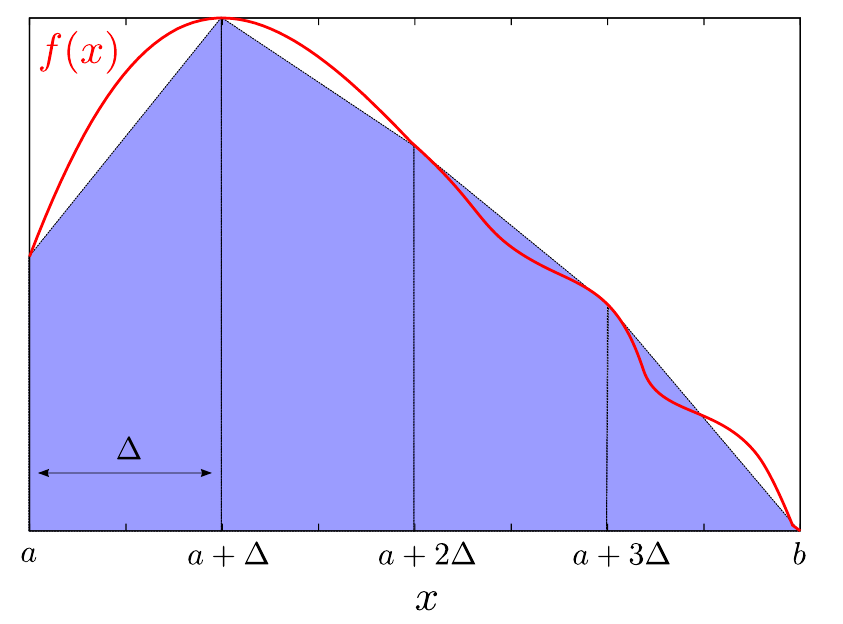
\includegraphics[width=8cm]{./Figures/20180227-trapezoidal-rule-example.png}
  \label{fig:ninc-nc-trapezoidal-rule}
%
%  \small{Source: PBOC.}
\end{figure}

见图\ref{fig:ninc-nc-trapezoidal-rule}所示,左数第$1$个梯形的面积等于
\begin{equation*}
  \frac{1}{2} \left[ f \left( a \right) + f \left( a + \Delta \right) \right] \cdot \Delta,
\end{equation*}

左数第$2$个梯形的面积等于
\begin{equation*}
  \frac{1}{2} \left[ f \left( a + \Delta \right) + f \left( a + 2 \Delta \right) \right] \cdot \Delta,
\end{equation*}
以此类推直到第$N=4$个梯形。将子区间中梯形的面积加总,可得
\begin{equation*}
\begin{split}
  \mathcal{I}_{N=4}^{trap} = &
    \frac{1}{2} \left[ f \left( a \right) + f \left( a + \Delta \right) \right] \cdot \Delta
    + \frac{1}{2} \left[ f \left( a + \Delta \right) + f \left( a + 2 \Delta \right) \right] \cdot \Delta \\
    & + \frac{1}{2} \left[ f \left( a + 2 \Delta \right) + f \left( a + 3 \Delta \right) \right] \cdot \Delta
    + \frac{1}{2} \left[ f \left( a + 3 \Delta \right) + f \left( a + 4 \Delta \right) \right] \cdot \Delta \\
    = & \left[
    \frac{1}{2} f \left( a \right)
    + f \left( a + \Delta \right)
    + f \left( a + 2 \Delta \right)
    + f \left( a + 3 \Delta \right)
    + \frac{1}{2} f \left( a + b \right)
    \right] \cdot \Delta,
\end{split}
\end{equation*}
扩展到更一般的$N \in \mathcal{N}$的情况,我们有$N$段梯形法则对$\int_{a}^{b} f \left( x \right) \, \mathrm{d} x$的近似为
\begin{equation}
  \label{eq:ninc-nc-trapezoidal-rule}
  \mathcal{I}_{N}^{trap} = \frac{1}{2} f \left( a \right) \cdot \Delta
  + \Delta \cdot \sum_{n=1}^{N-1} f \left( a + n \cdot \Delta \right)
  + \frac{1}{2} f \left( b \right) \cdot \Delta.
\end{equation}


梯形法则\eqref{eq:ninc-nc-trapezoidal-rule}成为对\eqref{eq:nint-num-integ-def}的又一种近似求积法则:
\begin{itemize}
  \item 求积点集合$\left\{ x_{n} \right\}_{n=1}^{N-1}$对应$x_{n} = a + n \cdot \Delta, \, n = 0,1,\ldots,N$,
  \item 求积权重集合$\left\{ w_{n} \right\}_{n=1}^{N}$对应
  \begin{equation*}
  w_{n} =
  \begin{cases}
  \frac{1}{2} \Delta, & n = 0, N, \\
  \Delta, & n = 1, 2, \ldots, N-1,
  \end{cases}
\end{equation*}
值得注意的是,比起矩形法则来,当利用梯形法则做近似求积时,需计算$N+1$个求积抽样点,比矩形法则多出的$1$个点为总区间中的末端$b$,对应$f(b)$。
\end{itemize}

\subsubsection{更高阶牛顿——寇特斯法则}
\label{sec:ninc-nc-higher-rule}
已知用$p=0$阶多项式(常数)近似子区间中的$f$,称矩形法则。用$p=1$阶多项式(斜线)近似,称梯形法则。那么我们可以进一步迭代计算更高阶$p > 1$的牛顿——寇特斯求积近似,方法如下
\begin{enumerate}
  \item 在子区间$\left[ x_{n}, x_{n+1} \right]$中,配$p+1$个等距离分布的点(包括子区间的起始点$x_{n}$和终结点$x_{n+1}$),将子区间分为$p$个部分。例如,
  \begin{itemize}
    \item 对$p=2$而言,配3个点$x_{n}, \frac{1}{2} \cdot \left[ x_{n} + x_{n+1} \right] , x_{n+1}$,
    \item 对$p=3$而言,配4个点$x_{n}, \frac{1}{3} \cdot \left[ x_{n} + x_{n+1} \right] , \frac{2}{3} \cdot \left[ x_{n} + x_{n+1} \right], x_{n+1}$,以此类推。
  \end{itemize}
  \item 在子空间中针对这$p+1$个配点,找到唯一的多项式$P(x)$以近似$f(x)$。例如,
  \begin{itemize}
    \item $p=0$,$P(x)$是个常数。矩形法则。
    \item $p=1$,$P(x)$是条斜线,连接子区间的两个端点$f \left( x_{n} \right), \, f \left( x_{n+1} \right)$。梯形法则。
    \item $p=2$,$P(x)$是一条经过如下3个点的抛物线,3个点的坐标依次为
    \begin{equation*}
      \begin{cases}
        \Big( x_{n}, f \left( x_{n} \right) \Big), \\
        \Big( x_{m}, f \left( x_{m} \right) \Big), \quad x_{m} \equiv \frac{x_{n} + x_{n+1}}{2}, \\
        \Big( x_{n+1}, f \left( x_{n+1} \right) \Big).
      \end{cases}
    \end{equation*}
    \item $p=3$,$P(x)$是一条经过如下4个点的曲线(图\ref{fig:ninc-nc-higher-p3}),4个点的坐标依次为
    \begin{equation*}
      \begin{cases}
        \Big( x_{n}, f \left( x_{n} \right) \Big), \\
        \Big( x_{m}, f \left( x_{m} \right) \Big), \quad x_{m} \equiv \frac{1}{3} \left( x_{n} + x_{n+1} \right), \\
        \Big( x_{m+1}, f \left( x_{m+1} \right) \Big), \quad x_{m+1} \equiv \frac{2}{3} \left( x_{n} + x_{n+1} \right), \\
        \Big( x_{n+1}, f \left( x_{n+1} \right) \Big),
      \end{cases}
    \end{equation*}
    \begin{figure}[htbp]
       \caption{3阶牛顿——寇特斯法则,对应子区间中的4个配点}
      \centering
      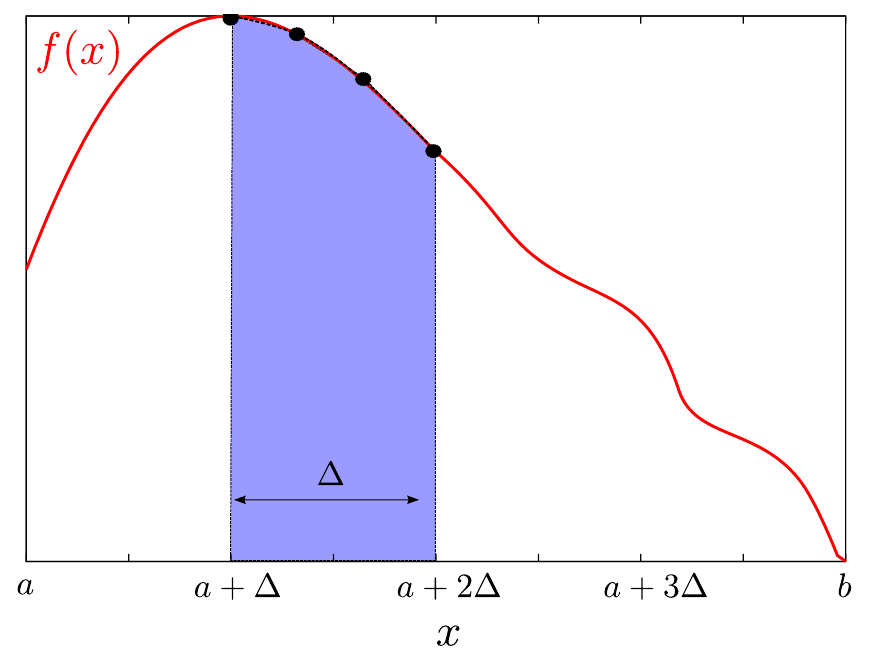
\includegraphics[width=8cm]{./Figures/20180227-nc-higher.png}
      \label{fig:ninc-nc-higher-p3}
    %
    %  \small{Source: PBOC.}
    \end{figure}
以此类推。无论哪一个例子中,$P(x)$都是这样一个多项式,其系数是抽样方程$f(x)$值的线性组合。
  \end{itemize}

  \item 从$x_{n}$到$x_{n+1}$对$P(x)$求积分,作为这个子区间内方程$f(x)$的近似。
  \item 将所有子区间内的近似方程组合起来,作为总区间中的最终近似求积法则。
\end{enumerate}

$p=2$时的牛顿——寇特斯求积,又称辛普森法则(Simpson's rule)\index{Simpson's (quadrature) rule \dotfill 辛普森(求积)法则}
\begin{equation}
  \label{eq:ninc-nc-simpson-rule}
  \mathcal{I}_{N}^{simp} =
  \sum_{n=0}^{N-1}
  \frac{\Delta}{6}
  \left[
  f \left( a + n \cdot \Delta \right)
  + 4 f \left( a + \left( n + \frac{1}{2} \right) \cdot \Delta \right)
  + f \left( a + \left( n + 1 \right)  \right) \cdot \Delta
  \right].
\end{equation}

\subsubsection{龙格现象}
\label{sec:ninc-nc-runge}
%20180227-Runge-phenomenon.png
一个自然出现的问题:更高阶的牛顿——寇特斯法则会不会带来更精确的近似解?很遗憾,答案是否定的。这是由于龙格现象(Runge phenomenon)\index{Runge phenomenon \dotfill 龙格现象}:当我们试图利用子空间中等距分布的点做更高阶多项式近似时,再查指点附近的多项式方程会出现较大幅度的震荡,从而影响最终求积估计的精确度,可参考\href{https://en.m.wikipedia.org/wiki/Runge%27s_phenomenon}{维基百科词条}。图\ref{fig:ninc-nc-higher-runge-phenomenon}中,蓝线和绿线分别表示$p=5$和$p=9$时的差值多项式近似,对应$N=6$。红线表示龙格方程(Runge function)。

\begin{figure}[htbp]
   \caption{龙格现象$(N=6)$}
  \centering
  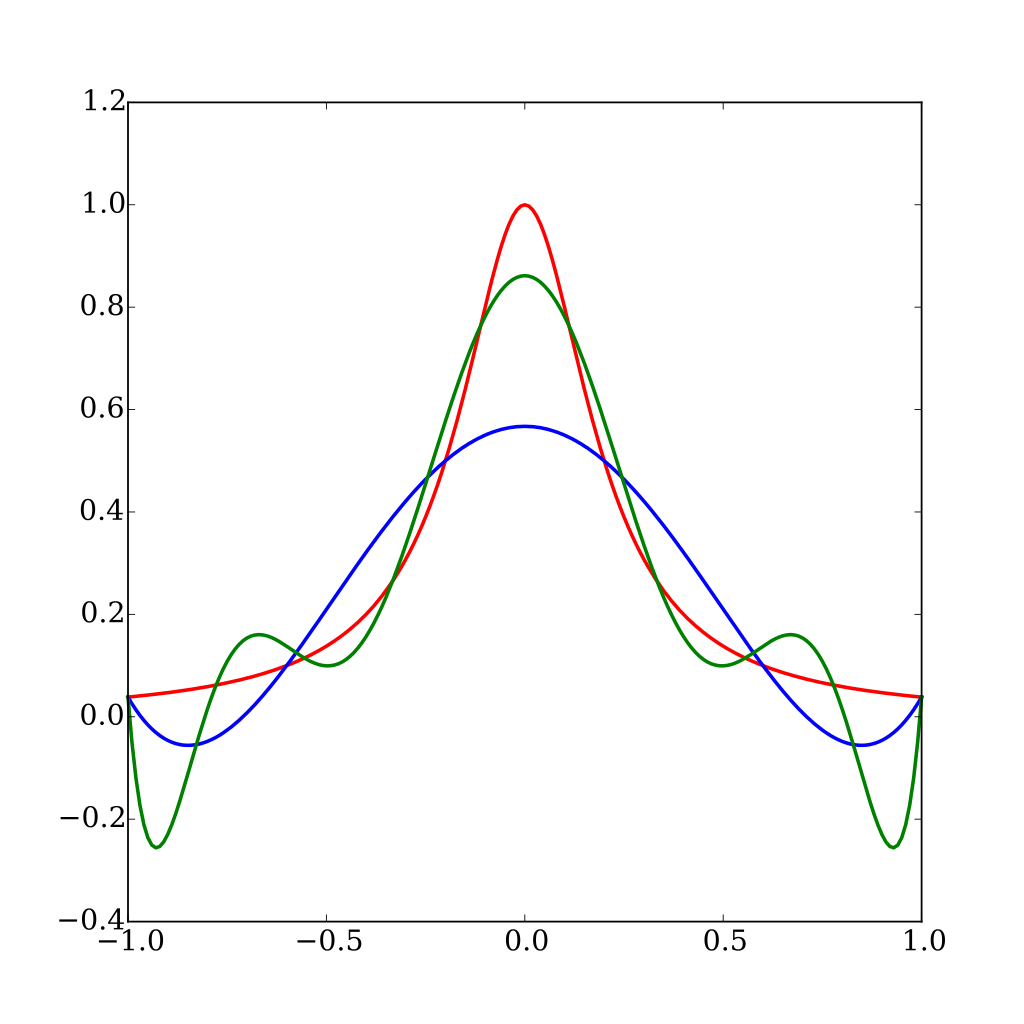
\includegraphics[width=8cm]{./Figures/20180227-Runge-phenomenon.png}
  \label{fig:ninc-nc-higher-runge-phenomenon}
%
%  \small{Source: PBOC.}
\end{figure}

\subsubsection{误差的收敛}
\label{sec:ninc-nc-error-convergence}
比较不同求积法则的优劣,可用启发式误差“分析”\footnote{加上引号是指,这种方法只是一种较为常用的检验措施,而不宜理解为某种严谨的学术性系统性表达。},观察近似误差随着配点数$N$增加的衰减速度。具体说来
\begin{enumerate}
  \item 考虑区间中某一宽度为$\Delta$的特定子区间,在其中用一个$p$阶多项式$P(x)$来近似$f$
  \begin{equation*}
    P(x) = c_{0} + c_{1} x + c_{2} x^{2} + \ldots + c_{p} x^{p}.
  \end{equation*}
  \item 那么子区间中存在一个点$x_{0}$,使得$f$围绕$x_{0}$做泰勒级数展开的前$p+1$项,与$P(x)$一致
  \footnote{例如
  \begin{itemize}
    \item $p=0$,矩形法则,$x_{0}$可以是子区间的起始点。
    \item $p=1$,梯形法则,$x_{0}$的存在性可由中值定理予以证明:$x_{n}$和$x_{n+1}$之间必然存在一点,该点上的方程值$f\left( x_{0} \right)$的导数,等于连接$f \left(x_{n} \right)$和$f \left( x_{n+1} \right)$两点的斜线的斜率。
    \item $p >1$,更高阶求和法则中$x_{0}$点存在性的证明,也可用类似思路证得。
  \end{itemize}
  }。
  可将$f$写成如下形式
  \begin{equation*}
    f(x) = \underbrace{
    c_{0} + c_{1} x + \ldots + c_{p} x^{p} }_{\equiv P(x)}
    + c_{p+1} x^{p+1} + \ldots.
  \end{equation*}
  \item 由此可见,原方程$f(x)$及其近似多项式$P(x)$之间的误差是一个从$p+1$阶开始的多项式
  \begin{equation*}
    f(x) - P(x) = c_{p+1} x^{p+1} + c_{p+2} x^{p+2} + \ldots,
  \end{equation*}
  \item 那么在这个子区间$\left[ x_{n}, x_{n+1} \right]$内的全部误差可求积得出
  \begin{equation*}
    \begin{split}
      \int \left[ f(x) - P(x) \right] \, \mathrm{d} x
      & = \int \left[
      c_{p+1} x^{p+1} + c_{p+2} x^{p+2} + \ldots \right] \, \mathrm{d} x \\
      & \propto \Delta^{p+2} + \text{更高阶项},
    \end{split}
  \end{equation*}
  最后一行是说,对$x^{p+1}$沿着某个宽度为$\Delta$的子区间求积,等于某个和$\Delta^{p+2}$成比例的值。
  \item 将一个子区间中的情况扩展到其他子区间,每个子区间中的误差项都与$\Delta^{p+2}$成定比例。更进一步地,由于$\Delta$与$N$反比例相关(N是整个区间中划分的子区间的数量)
  \begin{equation*}
    \Delta \sim \frac{1}{N},
  \end{equation*}
  那么每个子区间中的误差项可近似表示为
  \begin{equation*}
    \Delta \propto \frac{1}{N^{p+2}}.
  \end{equation*}
  \item 将$N$个子区间的误差项汇总
  \begin{equation}
    \varepsilon \propto \frac{N}{N^{p+2}} =  \frac{1}{N^{p+2}},
  \end{equation}
  例如矩形法则$(p=0)$的近似误差$\propto \frac{1}{N}$,梯形法则$(p=1)$的近似误差$\propto \frac{1}{N^{2}}$。可见误差与$N$成反比:$N$越大,划分的子区间数量越多,近似误差越小。
\end{enumerate}

举例,假定我们要用求积法则近似计算
\begin{equation*}
  \mathcal{I} = \int_{1}^{2} \log^{2} x \, \mathrm{d} x,
\end{equation*}
对应相对误差定义为$\varepsilon^{rel}$
\begin{equation*}
  \varepsilon^{rel} \equiv \frac{
  \big| \mathcal{I}_{N}^{approx} - \mathcal{I} \big|
  }{
  \mathcal{I}
  }
\end{equation*}

应用矩形法则和梯形法则,查看近似误差随着$N$增大的收敛情况如图\ref{fig:ninc-nc-error-convergence},可以看出

\begin{figure}[htbp]
   \caption{比较矩形法则和梯形法则下,近似误差随$N$值增大的收敛情况}
  \centering
  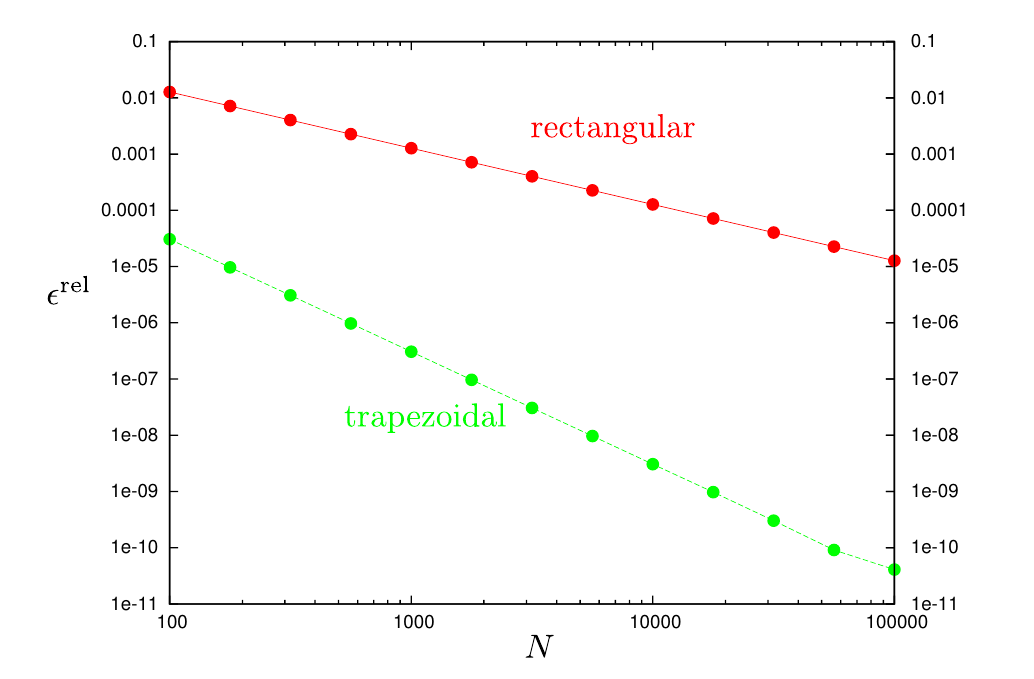
\includegraphics[width=10cm]{./Figures/20180227-nc-higher-error-convergence.png}
  \label{fig:ninc-nc-error-convergence}

  \small{原求积方程$\int_{1}^{2} \log^{2} x \, \mathrm{d} x$。}
\end{figure}

这两种方法代表的牛顿——寇特斯法则下误差项随着$N$而作线性收敛:
随着$N$增大$1,000$倍,矩形法则误差降低约$1,000$倍,$\Delta \varepsilon^{rect} \propto \frac{1}{\Delta N}$;梯形法则降低约$1,000,000$倍,$\Delta \varepsilon^{trap} \propto \frac{1}{ \left(\Delta N \right)^{2}}$。梯度法则优于矩形法则。

但图\ref{fig:ninc-nc-error-convergence}也揭示出牛顿——寇特斯法则的不足:即便是对于$\log^{2} x$这种很平滑的方程,梯形法则也需要大约$1,000$个样本,才能将总体误差控制在$10^{-6}$的水平上(为了达到类似的精度,矩形法则甚至需要$10^{6}$个样本)。从计算成本来看,牛顿——寇特斯法则恐怕不是最理想的方案,需要加以改进。如下文介绍的克伦肖——柯蒂斯法则,可以用少得多的样本量达到同样$10^{-6}$级别的误差水平,哪怕所处理的原方程更加复杂。我们做了一个小的数值计算实验来说明这个问题,见表\ref{tab:fourier-analysis-definition}。

\subsection{几个小技巧}
\label{sec:ninc-tips}
以牛顿——寇特斯法则为例,介绍几个小技巧。它们对其他如克伦肖——柯蒂斯法则也适用。

\subsubsection{无限区间求积}
\label{sec:ninc-tips-improper-integral}
有时会遇到求含有无限区间的积分问题如
\begin{equation*}
  \int_{0}^{\infty} f(x) \, \mathrm{d} x,
\end{equation*}
这需要我们先将区间$[0, \infty)$映射到一个有界区间内,如
\begin{equation*}
  x:[0, \infty) \mapsto u:[0,1],
\end{equation*}
然后再应用求解定积分的求积法则。映射的方法有很多种,其中之一是设
\begin{equation*}
  x \equiv \frac{u}{1-u}, \Rightarrow \mathrm{d} x = \frac{\mathrm{d} u}{\left( 1 - u \right)^{2}},
\end{equation*}
求积问题因此转换为
\begin{equation*}
  \int_{0}^{\infty} f(x) \, \mathrm{d} x = \int_{0}^{1} \frac{1}{\left( 1 - u \right)^{2}} f
  \left( \frac{u}{1 - u} \right) \, \mathrm{d} u.
\end{equation*}

需要指出的是,上式在转换之后,含有一个奇异点(singularity):$\lim_{u \rightarrow 1} f(x) \rightarrow \infty$。然而若是在前提假设中假定$f(x)$在$x \rightarrow \infty$处消失(这个假定是为了确保积分$\int_{0}^{\infty} f(x) \, \mathrm{d} x$收敛),则这一奇异点也就不存在了。

\subsection{求积中的可积奇异点问题}
\label{sec:ninc-nc-singularity}
除了上节提到的情况之外,还应该注意到,有些奇异点是可积的(integrable singular points)\index{integrable singular points \dotfill 可积奇异点},例如这个求积问题
\begin{equation}
  \label{eq:ninc-nc-singularity-example}
  \mathcal{I} = \int_{0}^{1} \frac{\exp(x)}{\sqrt{x}} \, \mathrm{d} x,
\end{equation}
方程在区间$(0,1]$内定义良好,除了起始点$0$的情况,称之为可积奇异点\footnote{注意区分可积和不可积奇异点。后者如积分方程$\int_{0}^{1} \frac{\exp (x)}{x} \, \mathrm{d} x $的起始点$0$的情况,此时积分不存在,因此无法估计。}。存在可积奇异点的积分方程并不是全都不能求解,针对具体问题的不同,有一些求解技巧可供选择。试举例如下。

\subsubsection{提取奇异点}
\label{sec:ninc-nc-singularity-isolation}
有时可以在积分中把奇异点单独提取出来做求积运算,如  \eqref{eq:ninc-nc-singularity-example}可以改写为
\begin{equation*}
  \begin{split}
    \mathcal{I} & =
    \underbrace{
    \int_{0}^{1} \frac{1}{\sqrt{x}} \, \mathrm{d} x
    }_{\eqqcolon \mathcal{I}_{1}}
    + \underbrace{
    \int_{0}^{1} \frac{
    \exp (x) -1
    }{\sqrt{x}} \, \mathrm{d} x
    }_{\eqqcolon \mathcal{I}_{2}}.
  \end{split}
\end{equation*}

其中$\mathcal{I}_{1}$可以用解析法求得
\begin{equation*}
  \mathcal{I}_{1} = \int_{0}^{1} \frac{1}{\sqrt{x}} \, \mathrm{d} x = \big| 2 \sqrt{x} \big|_{0}^{1} = 2.
\end{equation*}

含有可积奇异点的$\mathcal{I}_{2}$无法用解析法求解,但在区间起始点($=0$)处是非奇异的:这是由于,将被积方程沿着$x \rightarrow 0$做泰勒级数展开,可得
\begin{equation*}
  \begin{split}
    & \frac{
    \exp (x) -1
    }{\sqrt{x}}
    \approx \frac{
    x - \frac{1}{2}x^{2} + \frac{1}{6} x^{3} + \ldots
    }{
    \sqrt{x}
    } = x^{\frac{1}{2}} - \frac{1}{2}x^{\frac{3}{2}} + \frac{1}{6} x^{\frac{5}{2}} + \ldots, \\
    & \hookrightarrow \lim_{x \rightarrow 0}
    \frac{
    \exp (x) -1
    }{\sqrt{x}} \rightarrow 0,
  \end{split}
\end{equation*}
因此可用常规求积法则进一步近似求解$\mathcal{I}_{2}$。

\subsubsection{奇异点消除}
\label{sec:ninc-nc-singularity-cancellation}
若被积方程的分母中含有可积奇异点,那么
可以考虑用雅各比变换(Jacobian transformation)
%\index{Jacobian transformation \dotfill 雅各比变换}
。例如对\eqref{eq:ninc-nc-singularity-example},设
\begin{equation*}
  u \equiv \sqrt{x} \Rightarrow \mathrm{d} u = \frac{\mathrm{d} x}{2 \sqrt{x}},
\end{equation*}
求积运算因此变为
\begin{equation*}
  \int_{0}^{1} \frac{\exp(x)}{\sqrt{x}} \, \mathrm{d} x= 2 \int_{0}^{1} \exp \left( u ^{2} \right) \, \mathrm{d} u,
\end{equation*}
新的积分方程中没有奇异点,因此可进一步用常规数值求积法则来近似。

\subsubsection{Epsilon扩展}
\label{sec:ninc-nc-singularity-epsilon-extension}
如果可积奇异点无法利用前述两种方法消除,我们可以尝试加入一个平滑参数$\epsilon$。对应地,取极限$\lim \epsilon \rightarrow 0$以消除奇异点。如将\eqref{eq:ninc-nc-singularity-example}改写为
\begin{equation*}
  \mathcal{I}_{\epsilon} = \int_{0}^{1}
  \frac{
  \exp (x)
  }{
  \left( x^{2} + \epsilon^{2} \right)^{\frac{1}{4}}
  } \, \mathrm{d} x.
\end{equation*}

对于有限值的$\epsilon < \infty$,上式非奇异,并且$\lim_{\epsilon \rightarrow 0} \mathcal{I}_{\epsilon} \rightarrow \mathcal{I}$。

\subsubsection{适应性求积}
\label{sec:ninc-nc-singularity-adaptive-quadrature}
通常来说,被积方程在不同值域段的表现不同,如图  \ref{fig:ninc-nc-singularity-adaptive-quadrature}所示。如果我们应用梯形法则求解整个区间$[0,10]$内的积分,那么在子区间$[4,6]$中可能需要将宽度$\Delta$设的小一些,在$[0,4]$和$[6,10]$中将$\Delta$设的大一些。这就产生了适应性求积(adaptive quadrature)\index{adaptive quadrature \dotfill 适应性求积}的概念:随着子区间中方程变化的程度不同,应用不同的求积法则来做近似,以求近似精度和计算成本的平衡。举例来说,此时的梯形法则变为

\begin{figure}[htbp]
   \caption{适应性求积}
  \centering
  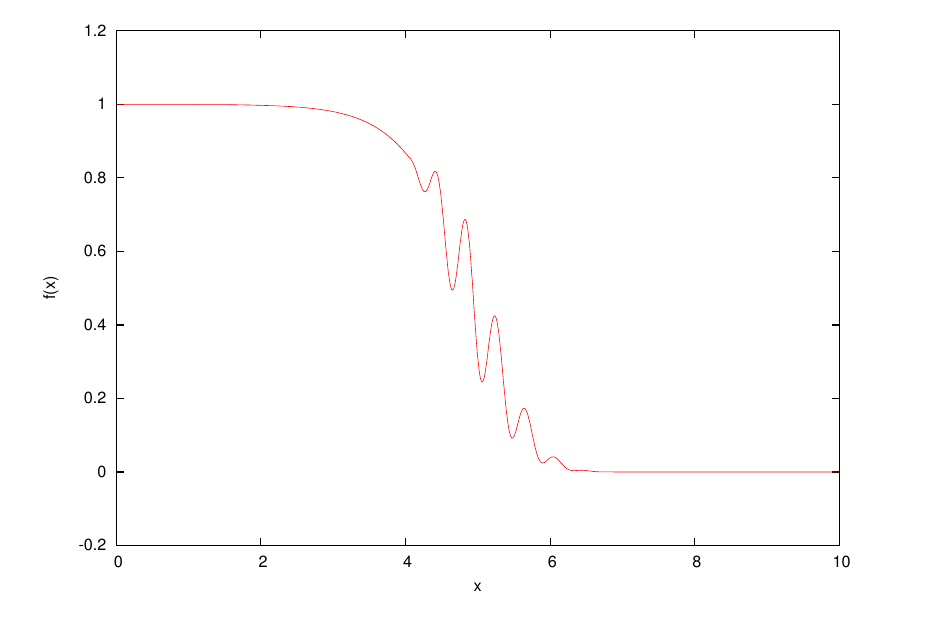
\includegraphics[width=10cm]{./Figures/20170227-nc-adaptive-quadrature.png}
  \label{fig:ninc-nc-singularity-adaptive-quadrature}
%
%  \small{Source: PBOC.}
\end{figure}

\subsection{克伦肖——柯蒂斯法则}
\label{sec:ninc-cc-rules}

如前文所述,牛顿——柯蒂斯求积法则(第\ref{sec:nint-nc-rule}节)的近似误差随着分段数$N$的衰减速度并不够令人满意;若是尝试利用更高阶多项式被积方程做近似,还会受到龙格现象的干扰。因此在实际应用中,常常并不会直接使用牛顿——柯蒂斯法则。一个更好的方案是克伦肖——柯蒂斯求积法则(Clenshaw-Curtis Rule)\index{Clenshaw-Curtis Rule \dotfill 克伦肖——柯蒂斯求积法则}。
在了解傅里叶分析(第\ref{sec:fourier-analysis}节)的基本要点之后,我们可以对这个法则有大致介绍。


\subsubsection{梯形法则的近似误差}
%傅里叶级数收敛分析}
%\label{sec:ninc-cc-trapezoidao-convergence}
\label{sec:ninc-cc-trapezoidal-error}
现在假定我们的目标是求解积分$\mathcal{I} = \int_{0}^{T} f(t) \, \mathrm{d} t$。根据梯形法则\eqref{eq:ninc-nc-trapezoidal-rule}可以做$N$个点的近似
\begin{equation}
  \label{eq:ninc-cc-trape-approx}
  I_{N}^{trap} = \frac{T}{N}
  \left\{
  \underbrace{
  \left[ \frac{1}{2} f(0) + \frac{1}{2} f(T) \right]
  }_{\eqqcolon \mathcal{A}}
  + \underbrace{
  \sum_{n=1}^{N-1} f \left( \frac{n T}{N} \right)
  }_{\eqqcolon \mathcal{B}}
  \right\},
\end{equation}
近似的精度与$N$有关:$N$越大,划分的点越多,近似越精确。我们将精度定义为误差项$\varepsilon_{N}^{trap}$
\begin{equation*}
  \varepsilon_{N}^{trap} = \left| \mathcal{I} - I_{N}^{trap} \right|.
\end{equation*}

现在引入傅里叶分析的概念。在实区间$[0,T]$中的方程$f(t)$,可写为傅里叶空间中的综合表达式
\begin{equation}
  \label{eq:ninc-cc-trape-fsynthesis}
  f(t) = \sum_{\nu = - \infty}^{\infty} \tilde{f}_{\nu} \exp \left( i \nu \omega_{0} t \right), \quad \omega_{0} \equiv \frac{2 \pi}{T},
\end{equation}
其中傅里叶级数的系数$\tilde{f}_{\nu}$值为
\begin{equation}
  \label{eq:ninc-cc-trape-fsynthesis-coef}
  \tilde{f}_{\nu} = \frac{1}{T} \int_{0}^{T} f(t) \exp \left( - i \nu \omega_{0} t \right) \mathrm{d} t.
\end{equation}

对$\mathcal{I}$做傅里叶变换可得
\begin{equation*}
  \begin{split}
    \mathcal{I} & = \int_{0}^{T} f(t) \, \mathrm{d} t = \int_{0}^{T} \sum_{\nu = -\infty}^{\infty} \tilde{f}_{\nu} \exp \left( i \nu \omega_{0} t \right) \, \mathrm{d} t \\
    & = \int_{0}^{T} \sum_{\nu = -\infty}^{\infty}
    \frac{1}{T} \int_{0}^{T} f(t) \exp \left( - i \nu \omega_{0} t \right) \, \mathrm{d} t \exp \left( i \nu \omega_{0} t \right) \, \mathrm{d} t \\
    & = T \tilde{f}_{0},
  \end{split}
\end{equation*}
即积分的值等于$T$个$\nu=0$时的系数$\tilde{f}_{\nu = 0}$值之和。

需要强调的时,在对$f(t)$利用梯形法则做牛顿——寇特斯求积时,我们并不知道系数$\left\{ \tilde{f}_{\nu} \right\}_{\nu}$的值——若是知道,也就不必再做傅里叶转换了。我们知道的是,存在一个关于被积方程$f(t)$的傅里叶综合表达形式\eqref{eq:ninc-cc-trape-fsynthesis},可供我们展开进一步的分析。

现在的任务是要将傅里叶综合式\eqref{eq:ninc-cc-trape-fsynthesis}代回梯形法则\eqref{eq:ninc-cc-trape-approx}。\eqref{eq:ninc-cc-trape-approx}RHS分为$\mathcal{A}$和$\mathcal{B}$两部分,
\begin{itemize}
  \item $\mathcal{A}$等于$t=0$时对\eqref{eq:ninc-cc-trape-fsynthesis}的计算:
  \begin{equation*}
    \mathcal{A} = \sum_{m=-\infty}^{\infty} \tilde{f}_{m},
  \end{equation*}
  分两种情况予以说明
  \begin{itemize}
    \item 当$f(t)$正好是一个$T$-周期方程时,$f(0)=f(T)$,显然这是正确的。
    \item 当$f(t)$的周期不等于$T$时,$\mathcal{A}$就等于设$t=0$时,对\eqref{eq:ninc-cc-trape-fsynthesis}的近似估计,见第\ref{sec:fourier-series-convergence}节。
  \end{itemize}
  \item $\mathcal{B}$的求和值,可以用一系列不同的$t=\frac{n T}{N}$来替代。
  \begin{equation*}
    \mathcal{B} = \sum_{n=1}^{N-1} \sum_{m=-\infty}^{\infty} \tilde{f}_{m} \exp \left( i m \omega_{0} \frac{n T}{N} \right).
  \end{equation*}
\end{itemize}

因此我们有
\begin{equation}
\begin{split}
  \label{eq:ninc-cc-trape-approx-m}
  I_{N}^{trap} & = \frac{T}{N}
  \left\{
  \mathcal{A} + \mathcal{B}
  \right\} = \frac{T}{N}
  \left\{
  \sum_{m=-\infty}^{\infty} \tilde{f}_{m}
  + \sum_{n=1}^{N-1} \sum_{m=-\infty}^{\infty} \tilde{f}_{m} \exp \left( i m \omega_{0} \frac{n T}{N} \right)
  \right\} \\
  & = \frac{T}{N} \sum_{n=0}^{N-1}
  \left\{
  \sum_{\nu = - \infty}^{\infty} \tilde{f}_{\nu} \exp
  \left(
  i \nu \omega_{0} \frac{n T}{N}
  \right)
  \right\}  = \frac{T}{N} \sum_{n=0}^{N-1}
  \left\{
  \sum_{\nu = - \infty}^{\infty} \tilde{f}_{\nu} \exp
  \left(
  2 \pi \frac{i \nu n }{N}
  \right)
  \right\},
\end{split}
\end{equation}

上式中引入一个新定义方程$K_{N} \left( \nu \right)$做进一步简化
\begin{equation}
  \label{eq:ninc-cc-trape-approx-knnu}
  I_{N}^{trap} = T \sum_{\nu = -\infty}^{\infty}
  \tilde{f}_{\nu} K_{N} \left( \nu \right),
\end{equation}

\begin{equation}
  \label{eq:ninc-cc-trape-approx-knnu-def}
  \begin{split}
    K_{N} \left( \nu \right) & \equiv \frac{1}{N} \sum_{n=0}^{N-1} \exp \left( 2 \pi \frac{i \nu n}{N} \right) \\
    & = \frac{1}{N} \left[ 1 + \xi + \xi^{2} + \ldots + \xi^{N-1} \right], \quad \xi \equiv \exp \left( 2 \pi \frac{i \nu}{N} \right),
  \end{split}
\end{equation}
$K_{N} \left( \nu \right)$的取值分为两种情况
\begin{itemize}
  \item $\nu=0$,或者$\nu$是一个$N$的整数倍是,有 $\xi = 1 \Rightarrow K_{N} \left( \nu \right) = 1$,
  \item $\nu \neq 0$且$\nu$不是$N$的整数倍时,有$\xi \neq 1$,以及
  \begin{equation*}
    K_{N} \left( \nu \right) \approx \frac{1}{N} \left[
    \frac{
    1 - \xi^{N}
    }{
    1 - \xi
    }
    \right] = \frac{1}{N} \frac{
    1 - \exp \left( 2 \pi i \nu \right)
    }{
    1 - \exp \left( \frac{2 \pi i \nu }{N}\right)
    } = 0.
  \end{equation*}
\end{itemize}

由此\eqref{eq:ninc-cc-trape-approx-knnu}进一步改写为
\begin{equation*}
  I_{N}^{trap} = T \sum_{\nu = -\infty}^{\infty}
  \tilde{f}_{\nu} K_{N} \left( \nu \right) = T \sum_{p = - \infty}^{\infty} \tilde{f}_{p N}, \quad p \in \mathcal{Z}.
\end{equation*}
可见对$[0,T]$区间中对周期方程求积问题$\int f(t) \, \mathrm{d} t$做$N$个点的梯形法则近似,其值与傅里叶级数的系数$\left\{ \tilde{f}_{\nu} \right\}_{\nu}$有关,但并不是全部系数,而仅仅是其中的一部分系数之和,具体说来是那些$N$的整数倍所对应的系数$\sum_{p} \tilde{f}_{p N}$,它们在傅里叶域中对应的傅里叶系数,是指频率为$N \omega_{0}$整数倍的若干条弦波曲线的傅里叶系数。尤其是,其中只有$\nu = 0$那条对应的项才是我们真正需要的;其余的部分都是误差项
\begin{equation*}
  I_{N}^{trap} =
  \underbrace{
  T \tilde{f}_{\nu = 0}
  }_{\mathcal{I}}
   +
   \underbrace{
   T \sum_{ p \neq 0} \tilde{f}_{p N}
   }_{\varepsilon_{N}^{trap}}, \Leftrightarrow \varepsilon_{N}^{trap} \equiv \left| \mathcal{I} - I_{N}^{trap} \right|,
\end{equation*}
$\varepsilon_{N}^{trap}$从而可以理解为第$\pm N$个,第$\pm 2N$个,$\ldots$个傅里叶级数的系数之和
\begin{equation}
  \label{eq:ninc-cc-trape-approx-error}
  \varepsilon_{N}^{trap} \equiv \left| \mathcal{I} - I_{N}^{trap} \right| = \left| \sum_{p = - \infty, p \neq 0}^{\infty} \tilde{f}_{p N} \right|.
\end{equation}

\subsubsection{连续非周期方程的傅里叶级数收敛}
\label{sec:ninc-cc-trapezoidao-convergence}

同样地,分析即使进展到\eqref{eq:ninc-cc-trape-approx-error}这一步,我们还是不知道傅里叶级数系数$\left\{ \tilde{f}_{p N}\right\}$的值,因而无法直接数值计算做近似求积。不过我们可以用傅里叶分析的平滑——衰减特性(第\ref{sec:fourier-smoothness-decay}节),来观察误差随着$N$的增大而衰减的速度有多快(收敛速度)。

随着被积方程$f(t)$是周期方程还是非周期方程,我们分两种情况来分析。首先考虑$f(t)$是平滑方程,但不满足$f(0)=f(T)$的情况。此时我们利用\eqref{eq:ninc-cc-trape-fsynthesis-coef}计算的傅里叶级数系数$\tilde{f}_{\nu}$是一个不连续方程。

为了在这种情况下做收敛分析,一个较原始的方案是\footnote{注意这里讨论的$T$-周期扩展方案较为直观易于理解,但精度上有所欠缺。在下文中我们将对$f(t)$做更精致的周期扩展。}\todo{reference}:将$[0,T]$中的这一段$f(t)$截取出来,以$T$周期为单位向前向后做重复扩展,所形成的一个新周期方程定义为$f^{per}(t)$,作为$f(t)$的$T$-周期扩展,见图\ref{fig:ninc-cc-trape-extension-convergence}。

\begin{figure}[htbp]
   \caption{非周期方程的$T$-周期扩展$t \in [0,1]$}
  \centering
  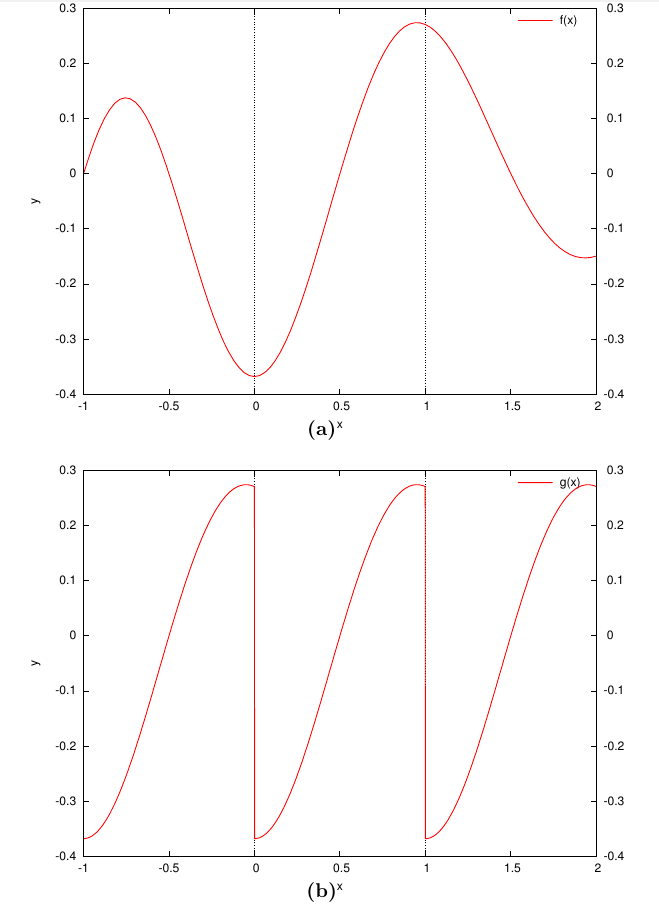
\includegraphics[width=12cm]{./Figures/20180306-fourier-period-extension.png}
  \label{fig:ninc-cc-trape-extension-convergence}
%
%  \small{Source: PBOC.}
\end{figure}

由佩利——维纳诸定理 (Theorem \ref{theorem:paley-wiener-theorems})可见,不连续方程$f(t)$的傅里叶系数的强度(magnitude) $\tilde{f}_{\nu}$,以等比于$\frac{1}{\nu}$的速度衰减。那么在理想状况下,根据\eqref{eq:ninc-cc-trape-approx-error},梯形法则的近似误差$\varepsilon_{N}^{trap}$
也应该以等比于$\frac{1}{N}$的速度衰减。然而实际上\eqref{eq:ninc-cc-trape-approx-error}中$\nu \in \mathcal{Z}$可以是正值也可以是负值,可能导致求和后的$\tilde{f}_{\nu}$被抵消掉。为了解决这个问题,我们在傅里叶系数求和式\eqref{eq:ninc-cc-trape-fsynthesis-coef}中区分$\nu>0$和$\nu <0$的情况,作分部积分\citep[Sec 2.9]{Boyd:2001wt}:
\begin{equation*}
  \begin{split}
    \tilde{f}_{\nu} & = \frac{1}{T} \int_{0}^{T} f(t) \exp \left( - i \nu \omega_{0} t \right) \mathrm{d} t \\
    & = \frac{1}{T} \left\{
    \frac{1}{i \nu \omega_{0}}
    \underbrace{
    \Big|
    f(t) \exp \left( - i \nu \omega_{0} t \right)
    \Big|_{0}^{T}
    }_{\eqqcolon \mathcal{A}}
    + \frac{1}{i \nu \omega_{0}}
    \int_{0}^{T} f^{'}(t) \exp \left( - i \nu \omega_{0} t \right) \, \mathrm{d} t
    \right\},
  \end{split}
\end{equation*}
其中
\begin{equation*}
  \begin{split}
    \mathcal{A} = \big| \cdot \big|_{0}^{T} = f(T)
    \underbrace{\exp \left( - i \nu \omega_{0} T \right)}_{=1} - f(0) \underbrace{\exp \left( - i \nu \omega_{0} 0 \right)}_{=1} = f(T) - f(0) \equiv \Delta f.
  \end{split}
\end{equation*}

那么我们有
\begin{equation*}
  \tilde{f}_{\nu} = \underbrace{
  \frac{\Delta f}{i \nu \omega_{0} T}
  }_{\eqqcolon \frac{C_{1}}{\nu}}
  + \frac{1}{i \nu \omega_{0}}
  \int_{0}^{T} f^{'}(t) \exp \left( - i \nu \omega_{0} t \right) \, \mathrm{d} t.
\end{equation*}

对上式再次分部积分,采用类似的思路,有
\begin{equation*}
  \tilde{f}_{\nu} = \underbrace{
  \frac{\Delta f}{i \nu \omega_{0} T}
  }_{\eqqcolon \frac{C_{1}}{\nu}}
  +
  \underbrace{
  \frac{\Delta f^{'}}{\left( i \nu \omega_{0} \right)^{2}}
  }_{\eqqcolon \frac{C_{2}}{\nu^{2}}}
   + \frac{1}{\left( i \nu \omega_{0} \right)^{2}} \int_{0}^{T} f^{''}(t) \exp \left( - i \nu \omega_{0} t \right) \, \mathrm{d} t,
\end{equation*}
其中$\Delta f^{'} \equiv f^{'}(T) - f^{'}(t)$。

继续进行下去可以看到,傅里叶系数$\tilde{f}_{\nu}$是一与$\nu$的幂次的倒数之和
\footnote{巧合的是,这恰好成为佩利——维纳诸定理(Theorem \ref{theorem:paley-wiener-theorems})的一种证明:如果$\Delta f=0$但$\Delta f^{'} \neq 0$,那么对$f(t)$的$T$-周期扩展中就同事含有连续的方程和不连续的倒数,那么其对应的不连续点就会出现在$p=1$处;进而由上面的扩展可得,随着$\left| \nu \right| \rightarrow \infty$,有$\left| \tilde{f}_{\nu} \right| \sim \frac{1}{\nu^{2}}$。
}
\begin{equation}
  \label{eq:ninc-cc-trape-fsynthesis-coef-boyd}
  \tilde{f}_{\nu} = \frac{C_{1}}{\nu}
  + \frac{C_{2}}{\nu^{2}}
  + \frac{C_{3}}{\nu^{3}}
  + \frac{C_{4}}{\nu^{4}} \ldots
\end{equation}

这样一来,若是取与正值$\nu$相对应的负值$- \nu$两两配对,将$\tilde{f}_{\nu}$和$\tilde{f}_{- \nu}$相加,则RHS中奇数项相互抵消,偶数项部分保留下来
\begin{equation}
  \label{eq:ninc-cc-trape-fsynthesis-coef-boyd-pair}
  \tilde{f}_{\nu} + \tilde{f}_{- \nu} =
  \frac{C^{'}_{2}}{\nu^{2}} + \frac{C^{'}_{4}}{\nu^{4}} + \ldots
\end{equation}
其中$C^{'}_{2} \equiv 2 C_{2}$,以此类推(常数项不重要,重要的是分母随着$\nu$值变化而表现出的渐进特性)。

将\eqref{eq:ninc-cc-trape-fsynthesis-coef-boyd-pair}代回\eqref{eq:ninc-cc-trape-approx-error}可得
\begin{equation*}
\begin{split}
    \varepsilon_{N}^{trap} & =  \left| \sum_{p = -\infty, p \neq 0}^{\infty} \tilde{f}_{p N} \right| =
    \left| \sum_{p = 1}^{\infty} \left( \tilde{f}_{p N} + \tilde{f}_{- p N} \right) \right| \\
    & = \frac{C^{'}_{2}}{N^{2}} \sum_{p=1}^{\infty} \frac{1}{p^{2}} = \frac{C^{'}_{2}}{N^{2}} \frac{\pi^{2}}{6},
\end{split}
\end{equation*}
忽略掉常数项可得,梯形法则下对非周期方程$f(t)$求积的近似误差$\varepsilon_{N}^{trap} \sim \frac{1}{N^{2}}$,即等比收敛至$\frac{1}{N^{2}}$。
